\documentclass[11pt]{beamer}
%\usetheme{CambridgeUS}
\usepackage[utf8]{inputenc}
\usepackage{amsmath}
\usepackage{amsfonts}
\usepackage{amssymb}
\usepackage{graphicx}
%\usepackage[outdir=./]{epstopdf}
\author{Hong Xiong}
%\title{}
%\setbeamercovered{transparent} 
\setbeamertemplate{navigation symbols}{} 
%\logo{} 
%\institute{} 
%\date{} 
%\subject{} 
\begin{document}

%\begin{frame}
%\tableofcontents
%\end{frame}

\begin{frame}
\includegraphics[width=\textwidth]{rssi_dis_fit.eps} 
\end{frame}

\begin{frame}
\includegraphics[width=\textwidth]{rssi_dis_fit_weighted.eps} 
\end{frame}

\begin{frame}
\centering
{\LARGE After extend the distance to 4.4m}
\end{frame}

\begin{frame}
\includegraphics[width=\textwidth]{rssi_dis_fit_4dot4m.eps} 
\end{frame}

\begin{frame}
\includegraphics[width=\textwidth]{rssi_dis_fit_weighted_4dot4m.eps} 
\end{frame}

\begin{frame}
\centering
{\LARGE After cutting the mean distance larger than 3m}
\end{frame}

\begin{frame}
\includegraphics[width=\textwidth]{cut_3m_rssi_dis_fit_4dot4m.eps} 
\end{frame}

\begin{frame}
\includegraphics[width=\textwidth]{cut_3m_rssi_dis_fit_weighted_4dot4m.eps} 
\end{frame}


\begin{frame}
\begin{itemize}
\item rssi distance direct mapping
\item rssi distance fitting
\item rssi distance weighted fitting
\item cut 3m direct mapping
\item cut 3m fitting
\item cut 3m weighted fitting
\end{itemize}
\end{frame}

\begin{frame}
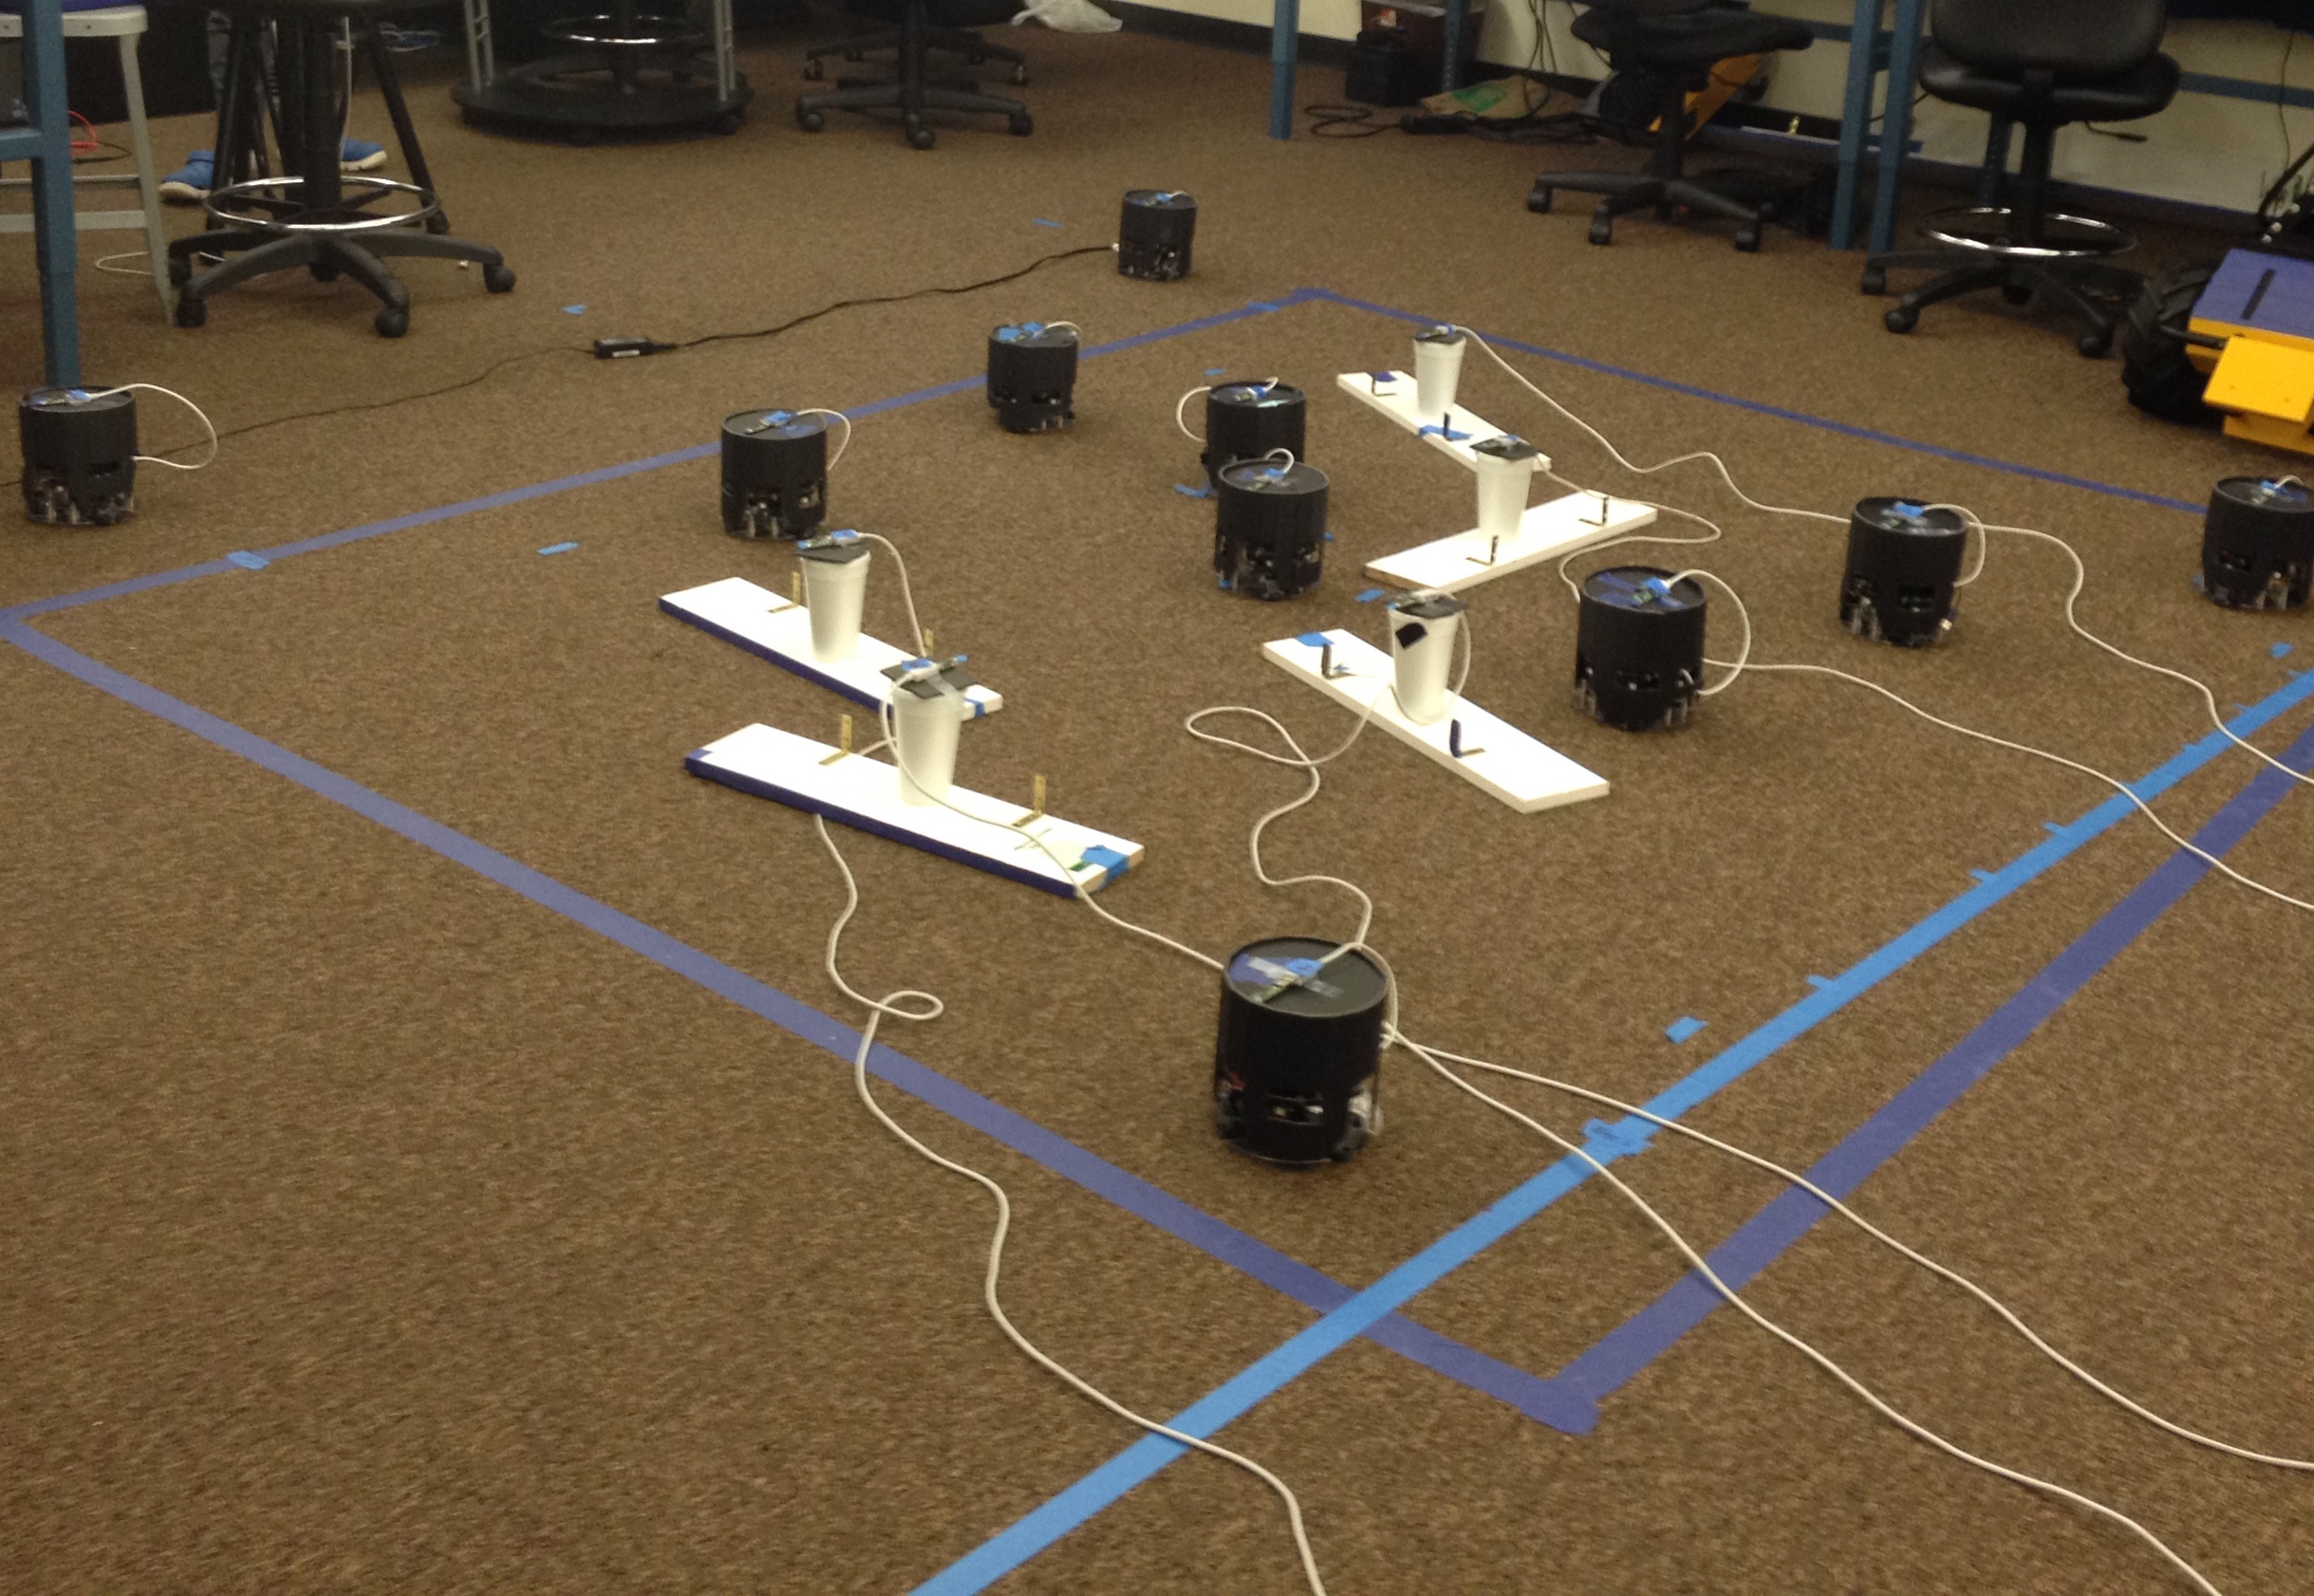
\includegraphics[width=\textwidth]{wolfbot_setup.jpg} 
\end{frame}

\begin{frame}
\includegraphics[width=\textwidth]{topo1.eps} 
\end{frame}

\begin{frame}
\frametitle{localization errors for kickloc (cut 3m treat outlier as boundary value)}
\tiny
\begin{tabular}{|c|c|c|c|c|c|c|}
\hline 
 & \multicolumn{6}{c|}{RSSI to Distance mapping model} \\ 
\hline 
Topology & direct  & fitting & weighted fitting & cut 3m direct & cut 3m fitting & cut 3m weighted fitting \\ 
\hline 
1 & 1.2288 & 0.5622 & 0.4823 & 1.1478 & 1.1623 & 1.2600 \\ 
\hline 
2 & 1.2942 & 1.4003 & 1.1707 & 1.3678 & 1.3309 & 1.2785 \\ 
\hline 
3 & 1.4390 & 1.1357 & 0.9791 & 1.2043 & 1.2858 & 1.3329 \\ 
\hline 
4 & 1.6591 & 1.3580 & 1.0879 & 1.5041 & 1.4235 & 1.5219 \\ 
\hline 
5 & 1.4182 & 1.1367 & 1.1893 & 1.2198 & 1.5674 & 1.9128 \\ 
\hline 
average & 1.4079 & 1.1186 & 0.9819 & 1.2887 & 1.3540 & 1.4612 \\ 
\hline 
\end{tabular} 
\end{frame}

\begin{frame}
\frametitle{localization errors for kickloc (cut 3m treat discard outlier)}
\tiny
\begin{tabular}{|c|c|c|c|c|c|c|}
\hline 
 & \multicolumn{6}{c|}{RSSI to Distance mapping model} \\ 
\hline 
Topology & direct  & fitting & weighted fitting & cut 3m direct & cut 3m fitting & cut 3m weighted fitting \\ 
\hline 
1 & 1.2288 & 0.5622 & 0.4823 & 1.1113 & 1.0564 & 1.0894 \\ 
\hline 
2 & 1.2942 & 1.4003 & 1.1707 & 0.9697 & 0.9849 & 1.0186 \\ 
\hline 
3 & 1.4390 & 1.1357 & 0.9791 & 1.1492 & 0.9733 & 1.1656 \\ 
\hline 
4 & 1.6591 & 1.3580 & 1.0879 & 1.4220 & 1.9286 & 1.4352 \\ 
\hline 
5 & 1.4182 & 1.1367 & 1.1893 & 1.2885 & 1.1299 & 1.6771 \\ 
\hline 
average & 1.4079 & 1.1186 & 0.9819 & 1.1881 & 1.2146 & 1.2772 \\ 
\hline 
\end{tabular} 
\end{frame}

\begin{frame}
\includegraphics[width=\textwidth]{rssi_dis_weighted_std_fitting.eps} 
\end{frame}

\begin{frame}
\frametitle{localization errors for kickloc (cut 3m treat discard outlier, distance std fitted)}
\tiny
\begin{tabular}{|c|c|c|c|c|c|c|}
\hline 
 & \multicolumn{6}{c|}{RSSI to Distance mapping model} \\ 
\hline 
Topology & direct  & fitting & weighted fitting & cut 3m direct & cut 3m fitting & cut 3m weighted fitting \\ 
\hline
1 & 1.3081 & 0.6765 & 0.5074 & 1.0748 & 1.0409 & 1.0713 \\
\hline
2 & 1.3366 & 1.4216 & 1.2271 & 0.9021 & 0.8996 & 0.9069 \\
\hline
3 & 1.3971 & 1.0839 & 0.9344 & 1.0996 & 0.9755 & 0.9869 \\
\hline
4 & 1.7022 & 1.1045 & 1.1086 & 1.4217 & 1.2172 & 1.2443 \\
\hline
5 & 1.6719 & 1.1286 & 1.0244 & 1.2712 & 1.1804 & 1.1905 \\
\hline
average & 1.4832 & 1.0830 & 0.9604 & 1.1539 & 1.0627 & 1.0800 \\
\hline 
\end{tabular} 
\end{frame}

\begin{frame}
 \frametitle{localization result for topo1 method6}
\includegraphics[width=0.8\textwidth]{final_mean_std_result_topo1_method6.eps} 
\end{frame}

\begin{frame}
 \frametitle{localization result for topo1 method6}
\includegraphics[width=\textwidth]{final_mean_result_topo1_method6.eps} 
\end{frame}

\begin{frame}
 \frametitle{time evolving result for topo1 method1}
\includegraphics[width=\textwidth]{time_evolving_topo1_method1.eps} 
\end{frame}

\begin{frame}
\frametitle{localization errors for kickloc when only leveraging beacon information}
\tiny
\begin{tabular}{|c|c|c|c|c|c|c|}
\hline 
 & \multicolumn{6}{c|}{RSSI to Distance mapping model} \\ 
\hline 
Topology & direct  & fitting & weighted fitting & cut 3m direct & cut 3m fitting & cut 3m weighted fitting \\ 
\hline 
1 & 1.5973 & 0.7827 & 0.7846 & 1.3661 & 1.4071 & 1.4873 \\
\hline 
2 & 1.1622 & 0.7455 & 0.8318 & 1.0589 & 1.2185 & 1.2768 \\
\hline 
3 & 1.3424 & 0.8064 & 0.8584 & 0.9084 & 1.2069 & 1.2656 \\
\hline 
4 & 1.7863 & 1.2275 & 1.0972 & 1.4245 & 1.6041 & 1.6898 \\
\hline 
5 & 1.6743 & 0.8378 & 0.8051 & 1.2402 & 1.4551 & 1.6199 \\
\hline 
average & 1.2190 & 0.8800 & 0.8754 & 1.1996 & 1.3783 & 1.4679 \\
\hline 
\end{tabular} 
\end{frame}

\begin{frame}
\frametitle{average localization errors for different algorithms }
\tiny
\begin{tabular}{|c|c|c|c|c|c|c|}
\hline 
 & \multicolumn{6}{c|}{RSSI to Distance mapping model} \\ 
\hline 
Algorithm & direct  & fitting & weighted fitting & cut 3m direct & cut 3m fitting & cut 3m weighted fitting \\ 
\hline 
KickLoc & 1.4079 & 1.1186 & 0.9819 & 1.2887 & 1.3540 & 1.4612 \\
\hline 
DV-distance & 1.1383 & 0.7624 & 0.8661 & 0.8438 & 1.0111 & 1.0975 \\
\hline
Min-Max & 0.6720 & 0.6679 & 0.6615 & 0.6543 & 0.6817 & 0.6975 \\
\hline
N-hop Lateration & 1.2285 & 0.9009 & 1.2003 & 1.0120 & 1.1691 & 1.2712 \\
\hline
\end{tabular} 
\end{frame}

%\begin{frame}
%\includegraphics[width=\textwidth]{dis_rssi_fit.eps} 
%\end{frame}
%
%\begin{frame}
%\includegraphics[width=\textwidth]{rssi_dis_reverse_fit.eps} 
%\end{frame}
%
%\begin{frame}
%\includegraphics[width=\textwidth]{rssi_dis_reverse_fit_cut_3m.eps} 
%\end{frame}

\begin{frame}
\includegraphics[width=\textwidth]{radiation_pattern_indoor.eps} 
\end{frame}

\begin{frame}
\includegraphics[width=\textwidth]{radiation_pattern_grass.eps} 
\end{frame}


\end{document}
